%\documentclass[handout]{ximera}
\documentclass[nooutcomes]{ximera}

\usepackage{gensymb}
\usepackage{tabularx}
\usepackage{mdframed}
\usepackage{pdfpages}
%\usepackage{chngcntr}

\let\problem\relax
\let\endproblem\relax

\newcommand{\property}[2]{#1#2}




\newtheoremstyle{SlantTheorem}{\topsep}{\fill}%%% space between body and thm
 {\slshape}                      %%% Thm body font
 {}                              %%% Indent amount (empty = no indent)
 {\bfseries\sffamily}            %%% Thm head font
 {}                              %%% Punctuation after thm head
 {3ex}                           %%% Space after thm head
 {\thmname{#1}\thmnumber{ #2}\thmnote{ \bfseries(#3)}} %%% Thm head spec
\theoremstyle{SlantTheorem}
\newtheorem{problem}{Problem}[]

%\counterwithin*{problem}{section}



%%%%%%%%%%%%%%%%%%%%%%%%%%%%Jenny's code%%%%%%%%%%%%%%%%%%%%

%%% Solution environment
%\newenvironment{solution}{
%\ifhandout\setbox0\vbox\bgroup\else
%\begin{trivlist}\item[\hskip \labelsep\small\itshape\bfseries Solution\hspace{2ex}]
%\par\noindent\upshape\small
%\fi}
%{\ifhandout\egroup\else
%\end{trivlist}
%\fi}
%
%
%%% instructorIntro environment
%\ifhandout
%\newenvironment{instructorIntro}[1][false]%
%{%
%\def\givenatend{\boolean{#1}}\ifthenelse{\boolean{#1}}{\begin{trivlist}\item}{\setbox0\vbox\bgroup}{}
%}
%{%
%\ifthenelse{\givenatend}{\end{trivlist}}{\egroup}{}
%}
%\else
%\newenvironment{instructorIntro}[1][false]%
%{%
%  \ifthenelse{\boolean{#1}}{\begin{trivlist}\item[\hskip \labelsep\bfseries Instructor Notes:\hspace{2ex}]}
%{\begin{trivlist}\item[\hskip \labelsep\bfseries Instructor Notes:\hspace{2ex}]}
%{}
%}
%% %% line at the bottom} 
%{\end{trivlist}\par\addvspace{.5ex}\nobreak\noindent\hung} 
%\fi
%
%


\let\instructorNotes\relax
\let\endinstructorNotes\relax
%%% instructorNotes environment
\ifhandout
\newenvironment{instructorNotes}[1][false]%
{%
\def\givenatend{\boolean{#1}}\ifthenelse{\boolean{#1}}{\begin{trivlist}\item}{\setbox0\vbox\bgroup}{}
}
{%
\ifthenelse{\givenatend}{\end{trivlist}}{\egroup}{}
}
\else
\newenvironment{instructorNotes}[1][false]%
{%
  \ifthenelse{\boolean{#1}}{\begin{trivlist}\item[\hskip \labelsep\bfseries {\Large Instructor Notes: \\} \hspace{\textwidth} ]}
{\begin{trivlist}\item[\hskip \labelsep\bfseries {\Large Instructor Notes: \\} \hspace{\textwidth} ]}
{}
}
{\end{trivlist}}
\fi


%% Suggested Timing
\newcommand{\timing}[1]{{\bf Suggested Timing: \hspace{2ex}} #1}




\hypersetup{
    colorlinks=true,       % false: boxed links; true: colored links
    linkcolor=blue,          % color of internal links (change box color with linkbordercolor)
    citecolor=green,        % color of links to bibliography
    filecolor=magenta,      % color of file links
    urlcolor=cyan           % color of external links
}

\title{Tenacity Paracity}
\author{Bart Snapp and Brad Findell}

\outcome{Learning outcome goes here.}

\begin{document}
\begin{abstract}
  We investigate city geometry parabolas.
\end{abstract}
\maketitle


\begin{problem} 
Remind me again, what is the definition of a \textit{parabola}?
\end{problem}
\vspace{0.5in}

\begin{problem}
Use the definition of a parabola and taxicab distance to sketch the city geometry parabola when the focus is the point $(2,1)$
and the directrix is $y=-3$. 
\begin{image}
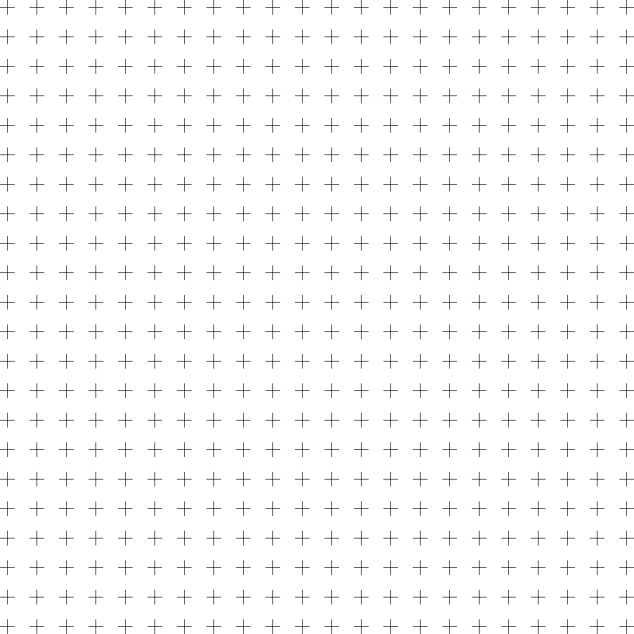
\includegraphics{complexPlane}
\end{image}
\end{problem}

\break
\begin{problem}
Comparing geometries with algebra. 
\begin{enumerate}
\item Use coordinate constructions to write an equation for the Euclidean geometry parabola with its focus at $(2,1)$ and its directrix being the line $y=-3$.  (Hint:  No need to simplify.  Just use the definition and set the distances equal to one another.)  
\vspace{0.5in}
\item Use your taxicab distance formula to write an equation for the city geometry parabola with its focus at $(2,1)$ and its directrix being the line $y=-3$.  
\vspace{0.5in}
\item Compare and contrast the two equations.  
\vspace{0.5in}
\item Use algebra of absolute value to show that the graph in the previous problem is the correct graph. 
 (Hint:  Consider three cases: $y>1$, $-3\leq y \leq 1$, and $y<-3$.)
\vfill
\end{enumerate}
\end{problem}

\break

\begin{problem}
Sketch the city geometry parabola when the focus is the point $(4,4)$
and the directrix is $y=-x$.
\begin{image}
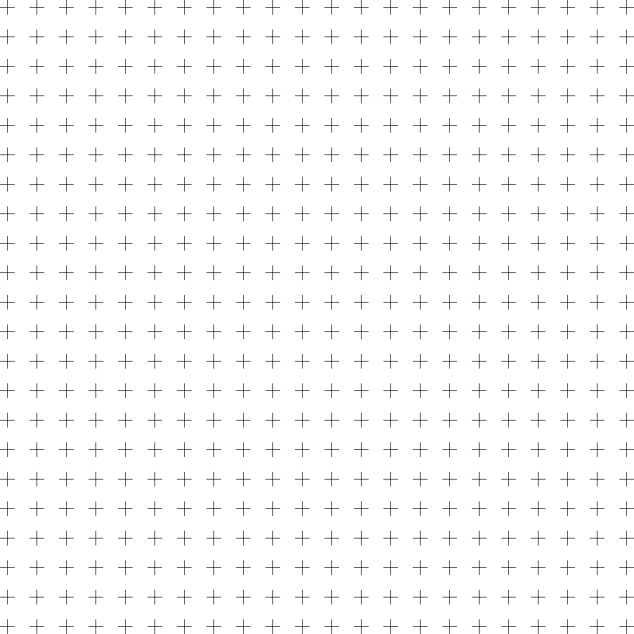
\includegraphics{complexPlane}
\end{image}
\end{problem}

\break

\begin{problem}
Sketch the city geometry parabola when the focus is the point $(0,4)$
and the directrix is $y=x/3$.
\begin{image}
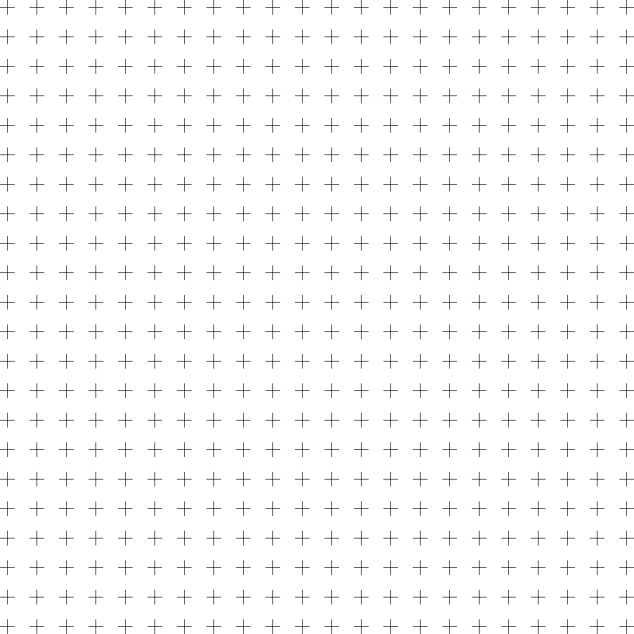
\includegraphics{complexPlane}
\end{image}
\end{problem}

\break

\fixnote{Use better numbers here.}
\begin{problem}
Sketch the city geometry parabola when the focus is the point $(4,1)$
and the directrix is $y=3x/2$.
\begin{image}
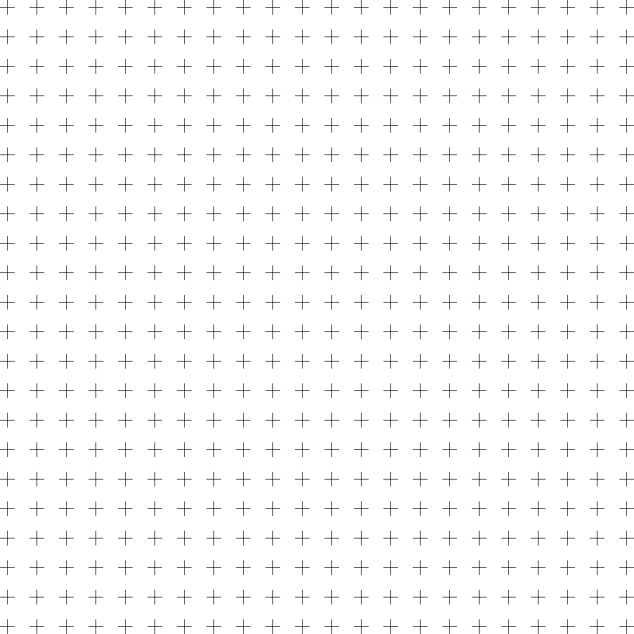
\includegraphics{complexPlane}
\end{image}
\end{problem}

\begin{problem}
Explain how to find the distance between a point and a line in city
geometry.
\end{problem}


\begin{problem}
Give instructions for sketching city geometry parabolas.
\end{problem}

\end{document}
